%% =====================================================================
%%  Robust analog two-qubit gates from deep reinforcement learning:
%%  an independent reproduction and family-resolved assessment
%%
%%  Preprint, REVTeX 4.2 (APS two-column style)
%%  Build:  pdflatex preprint ; bibtex preprint ; pdflatex x2
%% =====================================================================
\documentclass[aps,prx,twocolumn,superscriptaddress,nofootinbib,amsmath,amssymb,floatfix]{revtex4-2}

\usepackage{amsmath,amssymb,amsfonts,bm}
\usepackage{braket}
\usepackage{graphicx}
\usepackage{booktabs}
\usepackage{multirow}
\usepackage{siunitx}
\usepackage{xcolor}
\usepackage[colorlinks=true,linkcolor=blue,citecolor=blue,urlcolor=blue]{hyperref}

\graphicspath{{figures/}}

\sisetup{detect-all=true,range-phrase={--},range-units=single}

% ---- convenience macros -------------------------------------------------
\newcommand{\Ntgt}[2]{N(#1,#1,#2)}
\newcommand{\Ltot}{L_{\mathrm{tot}}}
\newcommand{\Hod}{\hat{H}_{\mathrm{od}}}
\newcommand{\Utgt}{U_{\mathrm{target}}}
\newcommand{\Fbar}{\overline{F}}
\newcommand{\snoise}{\sigma_{\mathrm{noise}}}
\newcommand{\strain}{\sigma_{\mathrm{train}}}
\newcommand{\Tsyn}{T_{\mathrm{syn}}}
\newcommand{\ns}{\,\mathrm{ns}}
\newcommand{\MHz}{\,\mathrm{MHz}}

\begin{document}

\title{Robust analog two-qubit gates from deep reinforcement learning:\\
an independent reproduction and family-resolved assessment}

\author{Francesco Giuseppe Minisini}
\email{fg.minisini@gmail.com}
\affiliation{Dipartimento di Fisica ``Aldo Pontremoli'', Universit\`a degli Studi di Milano, Via Celoria 16, 20133 Milano, Italy}

\date{\today}

\begin{abstract}
Reinforcement learning has been proposed as a unified route to analog quantum gate design, in which
accuracy, leakage suppression, runtime and robustness against stochastic control errors are optimized
jointly rather than sequentially. We report an independent, from-scratch reimplementation and critical
assessment of the Universal cost Function control Optimization (UFO) framework of Niu \emph{et al.}
[npj Quantum Inf.\ \textbf{5}, 33 (2019)] for the two-qubit gate family
$N(\alpha,\alpha,\gamma)=\exp[i(\alpha\sigma^x\sigma^x+\alpha\sigma^y\sigma^y+\gamma\sigma^z\sigma^z)]$
on a three-level-per-mode gmon model, including the second-order time-dependent Schrieffer--Wolff
leakage bound, the exact bandwidth filter, and trust-region policy optimization in a stochastic
control environment. Against a deliberately strong direct gradient (GRAPE-style, Adam) baseline
optimized on the same Hamiltonian and the same objective, we find that the qualitative claims of the
original work reproduce, while several quantitative ones do not. On a fixed nominal target the direct
optimizer \emph{outperforms} the policy-gradient controller in cost, runtime and leakage, so the value
of the learning formulation is not nominal optimality. Stochastic training is nonetheless
unambiguously effective as a robustness mechanism: against an otherwise identical agent trained
deterministically, the noise-trained policy attains higher average fidelity and lower fidelity
variance at \emph{every} noise strength in $\snoise\in[0.1,3.5]\MHz$. Its advantage over the
noise-aware direct optimizer, however, is confined to a neighbourhood of the training noise: the two
curves cross at $\snoise\approx1.3\MHz$, beyond which the direct optimizer is both more accurate and
more stable. Learned robustness is therefore local to the perturbation scale seen during training
rather than a global property, and the margins we measure ($1.4\times$ in infidelity over
deterministic RL at $1\MHz$) lie well below the one-to-two orders of magnitude originally reported. A
curriculum sweep across $\Ntgt{\alpha}{\pi/2}$ shows that the analog runtime advantage over optimal
gate synthesis is real but strongly structured, ranging from $16\%$ at the edges of the family to a
factor $2.8$ in a broad central basin and collapsing to a $2\ns$ solution at the hardware-aligned
point $\alpha=\pi/2$; sweeping the same family with the direct optimizer alone, however, yields
shorter pulses still, so the speedup belongs to analog pulse-level control rather than to the learning
method. We release the full parameter set needed to reproduce these numbers.
\end{abstract}

\maketitle

% =========================================================================
\section{Introduction}
\label{sec:intro}

A quantum algorithm is written as a sequence of logical unitaries, but a quantum processor executes
continuous-time dynamics generated by an experimentally accessible Hamiltonian. On pre-fault-tolerant
superconducting hardware the translation between the two is not a formality: coherence budgets,
calibration drift, waveform distortion and multilevel structure all limit which circuits can actually
be run~\cite{Krantz2019,Kjaergaard2020,Koch2022}. Quantum control is therefore not a fine-tuning layer
on top of compilation, but one of the binding constraints on usable computational depth.

This observation motivates a shift of perspective. Rather than decomposing a target two-qubit unitary
into a fixed universal gate alphabet and paying the runtime cost of every elementary operation, one
may attempt to realize it directly through a single shaped analog pulse that exploits the native
interactions of the device~\cite{Niu2019,Chen2014}. The appeal is concrete: if the target is well
aligned with the hardware's own entangling generator, the analog implementation can be substantially
shorter than any compiled circuit. The difficulty is equally concrete. Superconducting modes are
weakly anharmonic, so fast or aggressively modulated pulses drive population out of the computational
subspace~\cite{Motzoi2009,Werninghaus2021}; and the pulse that reaches the device is never the pulse
that was designed, because amplitudes fluctuate and Hamiltonian parameters are known only
approximately.

Niu \emph{et al.}~\cite{Niu2019} proposed to attack these requirements simultaneously rather than in
sequence. Their Universal cost Function control Optimization (UFO) framework combines three
ingredients: an analytic leakage estimate derived from a time-dependent Schrieffer--Wolff
transformation (TSWT), a scalar objective that adds leakage, boundary and runtime penalties to gate
infidelity, and a continuous-action reinforcement-learning (RL) formulation trained with trust-region
policy optimization (TRPO)~\cite{Schulman2015} in an environment where control noise is injected during
training. The reported outcome was strong: up to one order of magnitude lower average gate infidelity
than an RL agent trained without noise, roughly two orders of magnitude lower than a stochastic
gradient-descent baseline, about one order of magnitude smaller fidelity variance, and a factor-ten
runtime reduction relative to optimal gate synthesis on the subfamily $\Ntgt{\alpha}{\pi/2}$.

These are consequential claims, and they have been influential in establishing RL as a credible
language for robust pulse design~\cite{Bukov2018,Sivak2022,Khalid2023}. They have not, to our
knowledge, been subjected to an independent reimplementation. That is the purpose of this work.

\paragraph*{What this paper does.}
We rebuild the framework from scratch --- multilevel gmon simulator, second-order TSWT leakage
estimator, exact bandwidth filter, UFO objective, TRPO agent and stochastic environment --- and use it
to ask four questions. (i) Does the framework reproduce under an independent implementation, and with
what quantitative fidelity? (ii) How does the policy-gradient controller compare against a
\emph{strong} direct pulse optimizer, rather than a weak one, when both are given the same
Hamiltonian, the same constraints and the same objective? (iii) Is the improvement under noise
attributable to reinforcement learning as such, or specifically to stochastic training? (iv) How
robust are the conclusions to the free parameters that the original paper does not pin down, namely
the actor--critic architecture and the UFO weights?

\paragraph*{What we find.}
The qualitative picture survives; several numbers do not. Our central results are:
\begin{enumerate}
\item On the representative nominal target $\Ntgt{2.2}{\pi/2}$, a GRAPE-style Adam optimizer beats the
nominal TRPO controller on \emph{every} nominal metric --- total cost ($0.158$ vs $0.298$), runtime
($70\ns$ vs $116\ns$) and leakage ($2.8\times10^{-4}$ vs $1.6\times10^{-3}$). Policy-gradient control
is not intrinsically a better nominal pulse optimizer.
\item Stochastic training works, and the controlled comparison is unambiguous: the noise-trained agent
has higher average fidelity and lower fidelity variance than the deterministically trained agent at
\emph{every one} of the $3401$ noise strengths tested. Because the two share architecture, objective
and algorithm, this isolates stochastic \emph{training} as the operative ingredient.
\item That advantage is nonetheless local to the training scale, and smaller than originally reported.
Relative to the nominal agent the infidelity ratio falls from $3.8$ at $\snoise=0.1\MHz$ to $1.44$ at
$1\MHz$. Against the noise-aware Adam baseline the noise-trained policy wins only below
$\snoise\approx1.3\MHz$; beyond that crossover the direct optimizer is both more accurate and more
stable, and it is the slowest-degrading controller overall.
\item The runtime advantage over optimal gate synthesis is real across the entire family
$\Ntgt{\alpha}{\pi/2}$, but ranges from $16\%$ at the edges to $2.8\times$ in the central basin, with a
singular hardware-aligned point at $\alpha=\pi/2$ solved in $2\ns$. The advantage tracks alignment with
the native exchange interaction, exactly as the physical argument of Ref.~\cite{Niu2019} predicts.
\item It is not, however, a benefit of the learning method. Sweeping the same family with the direct
optimizer alone gives shorter pulses than the curriculum-trained policy at every target but
$\alpha=\pi/2$ (median $3.1\times$ over synthesis, against $1.5$--$2.0\times$), at comparable fidelity
and robustness. The speedup is a property of analog pulse-level control, not of reinforcement learning.
\end{enumerate}

Section~\ref{sec:framework} states the framework; Sec.~\ref{sec:methods} gives the implementation and
the complete parameter set; Sec.~\ref{sec:modelsel} fixes the free parameters through two sweeps;
Secs.~\ref{sec:single}--\ref{sec:runtime} present the nominal, robustness and runtime results;
Sec.~\ref{sec:discussion} confronts them with the original claims.

% =========================================================================
\section{Control framework}
\label{sec:framework}

\subsection{Physical model and control channels}
\label{sec:model}

The platform is the gmon architecture, sketched in Fig.~\ref{fig:gmon}: two weakly anharmonic
superconducting modes with local drive and frequency control, coupled through a flux-tunable
interaction~\cite{Chen2014}. The tunability of the coupling is what makes the platform interesting for
analog gate design, because the entangling interaction becomes a control resource rather than a fixed
background.

\begin{figure}[t]
\centering
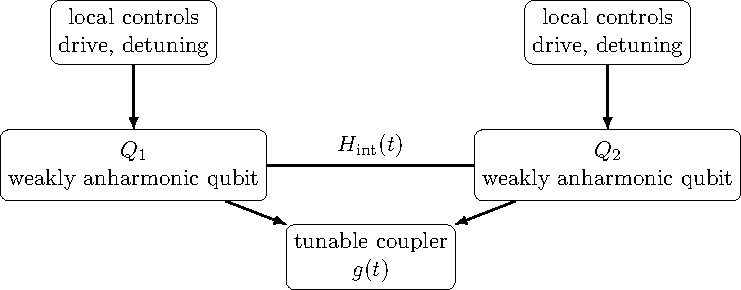
\includegraphics[width=\columnwidth]{gmon_architecture_schematic.pdf}
\caption{The gmon control setting. Two weakly anharmonic modes are driven locally and coupled through a
tunable interaction $g(t)$. Local addressability together with a time-dependent coupling gives the
seven control channels of Eq.~\eqref{eq:controls}.}
\label{fig:gmon}
\end{figure}

After circuit quantization, transformation to the interaction picture and a rotating-wave
approximation, the effective two-mode Hamiltonian is~\cite{Niu2019}
\begin{align}
\hat{H}_{\mathrm{RWA}}(t) =\;&
\frac{\eta}{2}\sum_{j=1}^{2}\hat{n}_{j}\bigl(\hat{n}_{j}-1\bigr)
+ g(t)\bigl(\hat{a}_{2}^{\dagger}\hat{a}_{1}+\hat{a}_{1}^{\dagger}\hat{a}_{2}\bigr)
\nonumber\\
&+\sum_{j=1}^{2}\delta_{j}(t)\hat{n}_{j}
\nonumber\\
&+\sum_{j=1}^{2} i f_{j}(t)\Bigl(\hat{a}_{j}e^{i\phi_{j}} - \hat{a}_{j}^{\dagger}e^{-i\phi_{j}}\Bigr),
\label{eq:hrwa}
\end{align}
with $\hat{n}_j=\hat{a}_j^\dagger \hat{a}_j$. The four terms carry distinct physical roles. The
anharmonicity $\eta$ breaks the harmonic ladder and makes the lowest two levels of each mode a usable
qubit; because $\eta$ is finite, the system stays intrinsically multilevel and leakage remains a real
error channel. The exchange term is the entangling resource. The detunings act diagonally and shape
relative phase accumulation. The drives generate local rotations. The available controls are therefore
\begin{equation}
\bm{u}(t)=\bigl\{g(t),\;\delta_1(t),\delta_2(t),\;f_1(t),f_2(t),\;\phi_1(t),\phi_2(t)\bigr\}.
\label{eq:controls}
\end{equation}

Projected onto the logical subspace, Eq.~\eqref{eq:hrwa} becomes
\begin{align}
\hat{H}_{\mathrm{qb}}(t)=\;&\frac{g(t)}{2}\bigl(\sigma_{1}^{x}\sigma_{2}^{x}+\sigma_{1}^{y}\sigma_{2}^{y}\bigr)
\nonumber\\
&+\sum_{j}\Bigl[\frac{\delta_{j}}{2}\sigma_{j}^{z}
- f_{j}\bigl(\sin\phi_{j}\,\sigma_{j}^{x}+\cos\phi_{j}\,\sigma_{j}^{y}\bigr)\Bigr],
\label{eq:hqb}
\end{align}
which shows that the coupling generates an $XY$-type entangler while the local channels supply
arbitrary single-qubit rotations --- enough for universal two-qubit control. Equation~\eqref{eq:hqb}
is an interpretive tool only; all dynamics in this work are propagated with the full multilevel
Eq.~\eqref{eq:hrwa}, because the whole point is that leakage must not be projected away.

\subsection{Subspaces and the TSWT leakage bound}
\label{sec:tswt}

In the Fock basis $\ket{n_1 n_2}$ the computational sector is
$\Omega_0=\mathrm{span}\{\ket{00},\ket{01},\ket{10},\ket{11}\}$ and the leading leakage sector is
$\Omega_1=\mathrm{span}\{\ket{02},\ket{20},\ket{12},\ket{21}\}$. Writing the physical space as
$\mathcal{H}=\bigoplus_\alpha \Omega_\alpha$ and decomposing
\begin{equation}
\hat{H}(t)=\hat{H}_0+\hat{H}_1(t)+\hat{H}_2(t),
\label{eq:decomp}
\end{equation}
the diagonal drift $\hat H_0$ sets the subspace energies, $\hat{H}_1$ is block-diagonal (evolution
within each sector) and $\hat{H}_2$ is block-off-diagonal (direct leakage). With $\Delta$ the minimum
gap between $\Omega_0$ and the leakage sectors and $\epsilon\sim\|\hat H_1\|\sim\|\hat H_2\|$ the
control scale, the regime of interest is $\epsilon/\Delta\ll1$.

The essential difficulty is that $\hat H_2$ cannot simply be switched off: the same controls that
produce the desired logical rotations also generate the inter-subspace coupling. Leakage suppression
is therefore a control problem, not a projection argument. The TSWT addresses it by moving to a
rotated frame $\ket{\tilde\psi}=e^{-\hat S(t)}\ket{\psi}$ with anti-Hermitian $\hat S$, in which
\begin{equation}
\hat{\mathbb{H}}(t)=-i\,\frac{d e^{-\hat{S}}}{dt}e^{\hat{S}} + e^{-\hat{S}}\hat{H}e^{\hat{S}}.
\label{eq:tswt}
\end{equation}
The first term is the price of a moving basis: in a driven system, leakage is generated not only by
direct coupling but also by the non-adiabatic motion of the frame itself. Expanding
$\hat S=\epsilon\hat S_1+\epsilon^2\hat S_2+\dots$ and cancelling block-off-diagonal terms order by
order leaves, at second order, a residual $\Hod=O(\epsilon^3/\Delta^2)$, from which the accumulated
coherent leakage over a gate of duration $T$ is bounded by
\begin{align}
\Ltot(T)\;\lesssim\;&
\frac{\|\Hod(0)\|}{\Delta(0)}+\frac{\|\Hod(T)\|}{\Delta(T)}
\nonumber\\
&+\int_{0}^{T}\frac{1}{\Delta(t)^{2}}\left\|\frac{d^{2}\Hod(t)}{dt^{2}}\right\|dt .
\label{eq:leakbound}
\end{align}
A derivation is summarized in Appendix~\ref{app:tswt}. The structure of Eq.~\eqref{eq:leakbound} is
what makes it useful for optimization rather than merely for diagnosis. The two boundary terms
penalize residual off-diagonal coupling at the pulse endpoints, and therefore push the controls toward
configurations where the dressed and bare bases coincide at $t=0$ and $t=T$. The integral term
penalizes rapid modulation of $\Hod$ and is the quantitative expression of the speed--leakage
trade-off: a pulse can be small in amplitude at every instant and still leak, if it changes too
quickly. Crucially, Eq.~\eqref{eq:leakbound} is written in terms of the Hamiltonian and its
derivatives, so it can be accumulated online during propagation instead of requiring a separate
population measurement at the end of the pulse.

\subsection{The UFO objective}
\label{sec:ufo}

\begin{figure}[t]
\centering

\includegraphics[width=\columnwidth]{ufo_cost_structure.pdf}
\caption{The UFO objective, Eq.~\eqref{eq:ufo}, scalarizes four competing physical requirements:
logical accuracy, accumulated leakage, boundary regularity and total runtime.}
\label{fig:ufostructure}
\end{figure}

Let $U(T)=\mathcal{T}\exp[-i\int_0^T \hat H_{\mathrm{RWA}}(t)dt]$ and let $U_{\mathrm{proj}}$ be its
restriction to $\Omega_0$. The gate fidelity with respect to $\Utgt$ is
\begin{equation}
F=\frac{1}{16}\bigl|\mathrm{Tr}\bigl(U_{\mathrm{proj}}^{\dagger}(T)\,\Utgt\bigr)\bigr|^{2},
\label{eq:fidelity}
\end{equation}
which equals $1$ exactly when the implemented gate matches the target up to a global phase. The full
objective adds three penalties to this term, as summarized in Fig.~\ref{fig:ufostructure}~\cite{Niu2019}:
\begin{align}
C(\chi,\beta,\mu,\kappa)=\;&
\chi\bigl[1-F\bigr]+\beta \Ltot+\kappa T
\nonumber\\
&+\mu\!\!\sum_{t\in\{0,T\}}\!\!\bigl[g(t)^2+f_1(t)^2+f_2(t)^2\bigr].
\label{eq:ufo}
\end{align}
The boundary term enforces vanishing envelopes at the pulse edges, which both permits clean gate
concatenation and reduces errors from deviations of the rotating-wave approximation; the linear
runtime penalty encodes the fact that long gates buy more exposure to decoherence and drift.

The design choice that matters here is that all of these are \emph{soft} constraints. Much earlier
leakage-mitigation work proceeded by disabling control channels or imposing structural restrictions on
the admissible pulse shape, which suppresses leakage at the price of controllability. UFO keeps every
channel available and penalizes undesirable behaviour instead, leaving the optimizer free to trade the
four objectives against one another. This also means the framework is modular: on a different platform
the individual terms can be replaced without changing the logic.

\subsection{Reinforcement-learning formulation}
\label{sec:rl}

The pulse is built sequentially. Time is discretized in steps $\Delta t$; the state presented to the
agent is a representation of the propagator accumulated so far, $s_n\sim U_n$; the action is the
control vector for the next interval,
$a_n=(g_n,\delta_{1,n},\delta_{2,n},f_{1,n},f_{2,n},\phi_{1,n},\phi_{2,n})$; and the environment
propagates
\begin{equation}
U_{n+1}=\exp\!\bigl[-i\Delta t(\hat{H}_{n+1}+\delta\hat{H}_{n+1})\bigr]U_n ,
\label{eq:envstep}
\end{equation}
where $\delta\hat H$ is the stochastic perturbation used in noisy training. The reward is the negative
running UFO cost, $r_n=-c_n$, so maximizing expected return minimizes the expected objective. An
episode terminates at $\min(T_{\max},T_{\mathrm{stop}})$, where $T_{\mathrm{stop}}$ is the first time
the cost falls below a threshold; the agent thus co-optimizes pulse shape \emph{and} stopping time,
which is a structural difference from fixed-horizon pulse optimization.

Using the accumulated unitary as the state is a deliberate choice: the agent reasons in terms of how
much of the target operation has already been built, rather than in terms of local control variables,
which matches the structure of gate synthesis.

Optimization uses TRPO~\cite{Schulman2015}, which maximizes the importance-weighted surrogate
\begin{equation}
\mathcal{L}(\bm{\theta})=\mathbb{E}_{\pi_{\bm\theta_{\mathrm{old}}}}\!\left[
\frac{\pi_{\bm{\theta}}(a|s)}{\pi_{\bm{\theta}_{\mathrm{old}}}(a|s)}\hat{A}(s,a)\right]
\;\;\text{s.t.}\;\;
\mathbb{E}_s\bigl[D_{\mathrm{KL}}\bigr]\le\delta_{\mathrm{KL}} .
\label{eq:trpo}
\end{equation}
The trust-region constraint matters here for a specific reason: the UFO reward couples four competing
terms and the environment is stochastic, so the landscape is irregular and a single over-large
gradient step can destroy previously learned behaviour. Constraining the step in distribution space
buys stability at the cost of speed.

Robustness enters through the environment rather than through an outer loop. In noise-optimized
training, Gaussian fluctuations are added to the control amplitudes at every step, so the objective
becomes an expectation over both the policy and the noise,
$J(\bm\theta)=-\mathbb{E}_{\tau,\xi}[C]$. Pulse trajectories that are fragile under small perturbations
earn poor average return and are disfavoured; stochastic training therefore acts as an implicit
regularizer. Throughout this paper we call \emph{nominal} an agent trained in the deterministic
environment and \emph{noise-optimized} one trained in the stochastic environment. They differ only in
the training distribution --- same architecture, same objective, same algorithm --- which is what makes
their comparison informative.

\subsection{Target family and synthesis reference}
\label{sec:targets}

Benchmarking uses the family
\begin{equation}
\Ntgt{\alpha}{\gamma}=\exp\!\bigl[i\bigl(\alpha\sigma_1^x\sigma_2^x+\alpha\sigma_1^y\sigma_2^y+\gamma\sigma_1^z\sigma_2^z\bigr)\bigr].
\label{eq:family}
\end{equation}
The equal $XX$ and $YY$ coefficients mirror the exchange structure of the gmon coupling, so the family
is deliberately close to the hardware's native interaction while remaining rich: up to single-qubit
rotations it contains SWAP, iSWAP, CNOT and CZ, as well as the fermionic SWAP and Givens rotations
that appear in Jordan--Wigner-mapped fermionic simulation~\cite{Niu2019}. Because it is continuously
parametrized, one can study an entire manifold of related targets rather than isolated cases.

The runtime reference is the optimal circuit decomposition of $\Ntgt{\alpha}{\gamma}$, which by the
Vatan--Williams construction requires three entangling gates and a small number of single-qubit
layers~\cite{VatanWilliams2004}. With the state-of-the-art gate times assumed in Ref.~\cite{Niu2019},
$T_{1q}=20\ns$ and $T_{\mathrm{CNOT}}=45\ns$, this gives
\begin{equation}
\Tsyn\approx 215\ns ,
\label{eq:tsyn}
\end{equation}
which we use unchanged as the compiled-implementation baseline.

% =========================================================================
\section{Numerical implementation}
\label{sec:methods}

\subsection{Simulator}

Each mode is truncated to three levels, giving $d_{\mathrm{phys}}=3^2=9$ and $d_{\mathrm{comp}}=4$.
Hamiltonians are kept in $\mathrm{rad}\,\mathrm{ns}^{-1}$ internally; one-step propagation uses exact
diagonalization of the Hermitian generator rather than a series expansion. The base anharmonicity is
$\eta=-200\MHz$, which also sets the gap scale entering Eq.~\eqref{eq:leakbound}. Control amplitudes
are bounded at $20\MHz$, well below $|\eta|$ so that the perturbative regime $\epsilon/\Delta\ll1$ is
respected, and phases are mapped to $[0,2\pi]$.

Before reaching the Hamiltonian, the piecewise-constant controls pass through the two-pole
double-exponential filter of Ref.~\cite{Niu2019}, implemented exactly: with
$a=\exp(-\pi B/f_s)$, $B=10\MHz$ the bandwidth and $f_s=1/\Delta t$ the sampling rate,
\begin{equation}
\tilde u_k=(1-a)^2 u_k + 2a\,\tilde u_{k-1} - a^2\,\tilde u_{k-2}.
\label{eq:filter}
\end{equation}
This is not cosmetic. It ensures that the optimizer cannot exploit arbitrarily sharp control
transitions that no waveform generator could produce, and it interacts directly with the
non-adiabatic term of the leakage bound.

The leakage estimator implements the second-order TSWT numerically: at each step it decomposes $H_t$
into $H_0,H_1,H_2$, solves for the generators $S_1$ and $S_2$ on the off-diagonal blocks, estimates
$\dot S_1,\dot S_2$ by finite differences, forms the residual
$H_{\mathrm{od}}^{(3)}=[H_1,S_2]+\tfrac{1}{3}[[H_2,S_1],S_1]-i\dot S_2$, and accumulates the boundary
and integral contributions of Eq.~\eqref{eq:leakbound} incrementally (Appendix~\ref{app:algo}). The
incremental form matters for cost: a naive implementation rescans the trajectory history at every step
and is $O(T^2)$ per rollout.

\subsection{Noise model}
\label{sec:noise}

At each step the realized control is $\bm{u}^{(\mathrm{noisy})}(t_k)=\bm{u}(t_k)+\bm{\xi}(t_k)$ with
$\bm\xi$ drawn independently from a zero-mean Gaussian of standard deviation $\snoise$. Perturbations
are applied to the coupling $g$, the detunings $\delta_{1,2}$ and the drive amplitudes $f_{1,2}$, and
additionally to the anharmonicity $\eta$; phases are left noise-free. Including $\eta$ is a
deliberate feature of the model: it probes sensitivity not only to imperfect pulse delivery but also
to uncertainty in a device parameter that the controller cannot actuate at all.

Training noise and evaluation noise are kept conceptually separate. The Adam baseline and the nominal
TRPO agent are optimized without perturbations and probed \emph{a posteriori}; the noise-optimized
agent sees the same perturbation model during training, at $\strain=1\MHz$.

\subsection{Controllers compared}
\label{sec:controllers}

\paragraph*{Direct gradient baseline (Adam).}
This is intended as a strong comparator, not a foil. For a fixed target and a fixed horizon $T$, the
full discretized trajectory $\{g_\ell,\delta_{j,\ell},f_{j,\ell},\phi_{j,\ell}\}_{\ell=0}^{N_T-1}$ is
optimized directly with Adam~\cite{Kingma2015} on the same multilevel model and the same objective
Eq.~\eqref{eq:ufo} --- a GRAPE-style direct pulse search~\cite{Khaneja2005,Koch2022} rather than a
literal reproduction of the canonical algorithm. Since the horizon is not a free variable of a single
run, the procedure is repeated over $T\in\{40,50,\dots,180\}\ns$ ($400$ Adam iterations each, learning
rate $0.03$) and the resulting plans are re-evaluated in a common deterministic simulator. The
baseline is therefore a family of fixed-horizon problems, whereas TRPO learns a variable-time policy;
this structural difference is precisely what makes the comparison informative.

\paragraph*{Nominal and noise-optimized TRPO.}
Both use the same actor--critic pair. The observation vectorizes the current $9\times9$ propagator into
real and imaginary parts and appends the normalized time index,
\begin{equation}
s_t=\bigl(\Re\,\mathrm{vec}(U_t),\;\Im\,\mathrm{vec}(U_t),\;t/T_{\max}\bigr),
\qquad d_{\mathrm{obs}}=163 .
\label{eq:obs}
\end{equation}
Actor and critic are multilayer perceptrons with hidden sizes $(64,32,32)$ and $\tanh$ activations, as
in Ref.~\cite{Niu2019}. The actor emits a mean $\mu_\theta(s_t)\in\mathbb{R}^7$ with a
state-independent trainable $\log\sigma$; raw actions $\tilde a_t=\mu_\theta+\sigma\odot\varepsilon_t$
are squashed by $\tanh$ into $[-1,1]^7$ and rescaled to physical bounds. The critic outputs a scalar
baseline for advantage estimation.

\paragraph*{Gate synthesis.}
The compiled reference of Eq.~\eqref{eq:tsyn}, used for runtime only.

\subsection{Metrics}
\label{sec:metrics}

Nominal quality is reported through the gate fidelity Eq.~\eqref{eq:fidelity}, the TSWT leakage
estimate $\Ltot$ with its boundary/integral split, the boundary penalty, the effective runtime and the
total cost Eq.~\eqref{eq:ufo}.

Robustness is characterized by two distinct quantities, and the distinction is worth stating
explicitly because they are often conflated. The first is the average fidelity of the
\emph{noise-averaged channel} $\mathcal{E}$, estimated from the Monte Carlo ensemble of noisy projected
unitaries $\{K_j\}$ through the standard formula~\cite{Nielsen2002}
\begin{equation}
\Fbar=\frac{\sum_{j}\mathrm{Tr}\bigl(\Utgt U_j^{\dagger}\Utgt^{\dagger}\,\mathcal{E}(U_j)\bigr)+d^{2}}{d^{2}(d+1)},
\qquad d=4,
\label{eq:favg}
\end{equation}
with $\{U_j\}$ a two-qubit Pauli basis. The second is the variance across realizations of the
per-shot gate fidelity,
\begin{equation}
\mathrm{Var}(F)=\mathbb{E}_{\xi}\bigl[(F_\xi-\mathbb{E}_\xi[F_\xi])^{2}\bigr].
\label{eq:fvar}
\end{equation}
A controller with good mean fidelity but large variance is experimentally fragile, so neither quantity
alone settles the question.

\subsection{Parameter set}
\label{sec:params}

Table~\ref{tab:config} collects every setting used. We report per-experiment values rather than a
single idealized configuration, because the model-selection sweeps deliberately ran under a reduced
budget and a looser stopping threshold than the production runs; conflating them would misstate what
was actually done.

\begin{table}[t]
\caption{Complete configuration. Values in the last two columns are the settings actually used for the
production runs and for the reduced-budget model-selection sweeps of Sec.~\ref{sec:modelsel}.}
\label{tab:config}
\footnotesize
\begin{ruledtabular}
\begin{tabular}{llcc}
Quantity & Symbol & Production & Sweeps \\
\colrule
\multicolumn{4}{l}{\textit{Physical model}}\\
Levels per mode & --- & 3 & 3 \\
Anharmonicity & $\eta$ & $-200\MHz$ & $-200\MHz$ \\
Control bound & $u_{\max}$ & $20\MHz$ & $20\MHz$ \\
Filter bandwidth & $B$ & $10\MHz$ & $10\MHz$ \\
Timestep & $\Delta t$ & $2\ns$ & $2\ns$ \\
Max gate duration & $T_{\max}$ & $180\ns$ & $180\ns$ \\
Runtime norm. & $T_{\mathrm{norm}}$ & $60\ns$ & $60\ns$ \\
\colrule
\multicolumn{4}{l}{\textit{UFO weights}}\\
Fidelity & $\chi$ & $10$ & swept \\
Leakage & $\beta$ & $10$ & $10$ \\
Boundary & $\mu$ & $0.2$ & swept \\
Runtime & $\kappa$ & $0.1$ & swept \\
\colrule
\multicolumn{4}{l}{\textit{TRPO}}\\
Hidden sizes & --- & $(64,32,32)$ & swept \\
Trust region & $\delta_{\mathrm{KL}}$ & $0.01$ & $0.01$ \\
Discount & $\gamma_{\mathrm{RL}}$ & $0.99$ & $0.99$ \\
GAE parameter & $\lambda$ & $0.97$ & $0.97$ \\
CG iters / damping & --- & $10$ / $0.1$ & $10$ / $0.1$ \\
Initial exploration & $\log\sigma_0$ & $-0.5$ & $-1.0$ \\
Value lr / epochs & --- & $10^{-3}$ / $50$ & $10^{-3}$ / $50$ \\
Episodes / batch & --- & $5000$\footnotemark[1] & $5000$ \\
Policy iterations & --- & $115$\footnotemark[2] & $20$ \\
Stopping cost & $C_{\mathrm{term}}$ & $0.30$\footnotemark[3] & $0.40$ \\
Training noise & $\strain$ & $1\MHz$ & $1\MHz$ \\
\colrule
\multicolumn{4}{l}{\textit{Adam baseline}}\\
Iterations per horizon & --- & $400$ & --- \\
Learning rate & --- & $0.03$ & --- \\
Horizon grid & --- & \multicolumn{2}{c}{$40$--$180\ns$, step $10\ns$}\\
\colrule
\multicolumn{4}{l}{\textit{Robustness evaluation}}\\
Noise grid & $\snoise$ & \multicolumn{2}{c}{$0.1$--$3.5\MHz$, step $0.001$}\\
Samples per $\snoise$ & --- & \multicolumn{2}{c}{$60$}\\
Smoothing (mean / var) & --- & \multicolumn{2}{c}{EWMA $50$ / $80$}\\
\end{tabular}
\end{ruledtabular}
\footnotetext[1]{$4000$ for the curriculum runtime sweep of Sec.~\ref{sec:runtime}.}
\footnotetext[2]{Up to $150$ per target in the curriculum sweep.}
\footnotetext[3]{$0.40$ in the curriculum sweep, which also uses it as the advancement threshold.}
\end{table}

% =========================================================================
\section{Fixing the free parameters}
\label{sec:modelsel}

Two ingredients of the framework are not determined by the physics: the capacity of the actor--critic
networks and the relative weights in Eq.~\eqref{eq:ufo}. Both could silently drive the comparisons
that follow, so we fix them first, on the representative target $\Ntgt{2.2}{\pi/2}$, under a reduced
budget and before any production run.

\subsection{Actor--critic architecture}
\label{sec:arch}

We swept five hidden-layer layouts of comparable scale, three seeds each, at $20$ policy iterations and
$5000$ episodes per batch (Table~\ref{tab:arch}). Selection was not made on total cost alone, because
a network can reach a favourable cost by trading leakage against fidelity or by settling on an
unnecessarily long pulse; we therefore tracked nominal fidelity, leakage, runtime and robustness at
$\snoise=1\MHz$ simultaneously.

\begin{table}[t]
\caption{Architecture sweep on $\Ntgt{2.2}{\pi/2}$, averaged over three seeds. Best value in each
column in bold.}
\label{tab:arch}
\begin{ruledtabular}
\begin{tabular}{lccccc}
Hidden sizes & $\overline{C}_{\mathrm{eval}}$ & $\overline{F}_{\mathrm{eval}}$ & $\Fbar_{\sigma=1}$ & $\overline{T}$ (ns) & $\overline{L}$ ($10^{-4}$)\\
\colrule
$(64,64,64)$      & \textbf{0.3584} & 0.9941          & \textbf{0.9637} & \textbf{106.7} & 4.05 \\
$(64,32,32)$      & 0.3592          & \textbf{0.9950} & 0.9622          & 111.3          & 3.67 \\
$(64,64,64,32)$   & 0.3626          & 0.9926          & 0.9604          & 107.3          & 4.17 \\
$(128,64,32)$     & 0.3630          & 0.9920          & 0.9616          & \textbf{106.7} & 4.22 \\
$(128,64,32,32)$  & 0.3691          & 0.9906          & 0.9589          & 110.7          & \textbf{3.56} \\
\end{tabular}
\end{ruledtabular}
\end{table}

\begin{figure}[t]
\centering
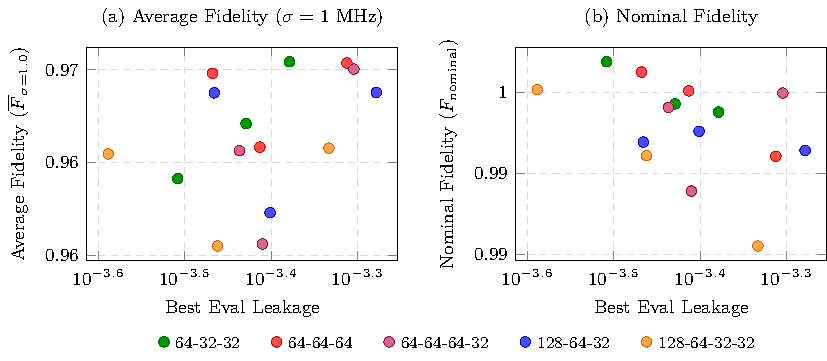
\includegraphics[width=\columnwidth]{architecture_sweep_pareto_combined.pdf}
\caption{Architecture trade-offs: evaluation leakage against (a) average fidelity at $\snoise=1\MHz$
and (b) nominal fidelity. Leakage minimization is not a proxy for robustness --- the layout with the
lowest leakage, $(128,64,32,32)$, has the worst aggregate cost and the weakest robustness.}
\label{fig:archpareto}
\end{figure}

Two conclusions follow. First, architecture is not neutral: moderate changes in width and depth
produce measurable differences in the final trade-off. Second, the dependence is not monotonic. The
deepest model tested achieves the \emph{lowest} mean leakage of the sweep and simultaneously the
\emph{worst} aggregate cost, the weakest robustness and the lowest nominal fidelity
(Fig.~\ref{fig:archpareto}). Minimizing one term of a multi-objective cost is not a selection
principle.

The best aggregate performer is $(64,64,64)$, but its margin over the paper layout $(64,32,32)$ is
$0.2\%$ in evaluation cost, and $(64,32,32)$ is in fact better in mean nominal fidelity and mean
leakage. Given a margin that small, and a sweep run under a deliberately reduced budget --- which makes
this a comparison of practical trainability rather than of asymptotic capacity --- we retain the paper
architecture $(64,32,32)$ for all production runs. This maximizes comparability with
Ref.~\cite{Niu2019} at negligible empirical cost.

\subsection{Sensitivity to the UFO weights}
\label{sec:weights}

The weights in Eq.~\eqref{eq:ufo} are part of the physical definition of the problem, not optimizer
settings, so they deserve separate treatment. We swept
$\chi\in\{5,10,20\}$, $\mu\in\{0.1,0.2,0.4\}$, $\kappa\in\{0.05,0.1,0.2,0.4\}$ at fixed $\beta=10$
(36 configurations, two seeds each). Holding $\beta$ fixed makes the sweep a study of the ratios
$\chi/\beta$, $\mu/\beta$, $\kappa/\beta$, which is the physically meaningful reading and keeps the
design tractable.

\begin{figure}[t]
\centering

\includegraphics[width=\columnwidth]{ufo_weight_sweep_robustness.pdf}
\caption{Sensitivity of the average fidelity at $\snoise=1\MHz$ to the UFO weights, shown separately
for the fidelity weight $\chi$, the boundary weight $\mu$ and the runtime weight $\kappa$. Underweighting
fidelity ($\chi=5$) opens a failure mode near $\Fbar\approx0.82$; $\mu=0.4$ is strongly bimodal;
$\kappa$ has almost no effect in this fixed-horizon regime.}
\label{fig:ufoweights}
\end{figure}

A methodological caveat governs the whole sweep: the best evaluation cost is \emph{not} a valid
selection criterion across configurations, because different weights define different scalarizations
and their numerical costs are not commensurable. Since all runs here terminate at the same evaluation
time of $180\ns$, increasing $\kappa$ mostly adds a rigid offset. We therefore compare on physical
quantities only --- nominal fidelity, leakage, and robustness at $\snoise=1\MHz$.

The fidelity weight has the clearest effect (Fig.~\ref{fig:ufoweights}). At $\chi=5$ the distribution
is broad and several runs collapse to $\Fbar\approx0.81$--$0.83$; at $\chi=10$ and $\chi=20$ it tightens
around $0.92$--$0.95$. Underweighting logical accuracy relative to leakage lets the optimizer settle
for controls that are clean but simply not the right gate. The boundary weight behaves
non-monotonically: $\mu=0.2$ gives the best median trade-off, $\mu=0.1$ leaves slightly more leakage,
and $\mu=0.4$ becomes strongly bimodal, producing both some of the best runs of the sweep and its worst
lower-tail failures. Larger $\mu$ does reduce the leakage proxy on average --- the lowest-leakage region
is often at $\mu=0.4$ --- but this does not translate into better robust control, which is the same
lesson the architecture sweep taught. The runtime weight $\kappa$ is nearly inert here, for the
structural reason noted above; its influence reappears in Sec.~\ref{sec:runtime}, where gate duration
is the observable rather than a fixed boundary condition.

The Pareto-favourable region is occupied jointly by $(\chi,\mu)\approx(10,0.2)$ and
$(\chi,\mu)\approx(20,0.4)$, with the latter marginally ahead. Given two seeds and a small budget, that
margin does not justify departing from the reference scalarization, so we retain
\begin{equation}
(\chi,\beta,\mu,\kappa)=(10,10,0.2,0.1)
\label{eq:weights}
\end{equation}
throughout. The useful conclusion is not the choice itself but its two components: the weights matter,
in a physically interpretable way, and the original values sit close to the best region in an
independent implementation.

% =========================================================================
\section{Single-target benchmark}
\label{sec:single}

All controllers are first compared on
\begin{equation}
\Utgt=\Ntgt{2.2}{\pi/2},
\label{eq:target}
\end{equation}
a target that is neither near-identity nor a degenerate special case, that sits in the family used for
the original robustness analysis, and that isolates optimizer differences by holding target difficulty
fixed.

\subsection{Direct gradient baseline}
\label{sec:adam}

\begin{figure}[t]
\centering

\includegraphics[width=\columnwidth]{adam_single_target_horizon_sweep.pdf}
\caption{Adam baseline on $\Ntgt{2.2}{\pi/2}$ versus gate horizon. (a) Nominal total cost, with the
optimum at $70\ns$ and the plan selected by the noisy objective at $60\ns$ both marked. (b) Boundary
and runtime penalties. (c) Nominal fidelity and total leakage. The optimum arises from the
simultaneous collapse of the boundary term and the rise in fidelity; longer horizons saturate in
fidelity and are penalized by runtime.}
\label{fig:adamsweep}
\end{figure}

Under deterministic re-evaluation the best Adam solution is at $T^\star=70\ns$, with nominal cost
$0.1576$, fidelity $0.99662$, total leakage $2.82\times10^{-4}$ and boundary penalty
$4.28\times10^{-3}$. Direct pulse optimization thus reaches fidelity comfortably above $99\%$ with
leakage in the $10^{-4}$ regime --- exactly the scale the leakage-aware objective is designed to
produce.

The horizon dependence (Fig.~\ref{fig:adamsweep}) is more informative than the optimum itself. Very
short pulses fail badly: fidelity drops to $0.726$ at $40\ns$ and $0.882$ at $50\ns$, while the
boundary penalties stay very large ($0.399$ and $0.357$). Notably, the leakage remains in the same
$10^{-4}$ band throughout this regime. The failure mode of ultra-short solutions is therefore
\emph{not} a leakage blow-up but the impossibility of satisfying accuracy and boundary regularity
simultaneously under strong time compression --- the speed--smoothness tension implicit in
Eq.~\eqref{eq:leakbound}. This is visible sharply between $60$ and $70\ns$: fidelity rises from $0.982$
to $0.997$, the boundary term collapses from $9.75\times10^{-2}$ to $4.28\times10^{-3}$, total cost
falls from $0.381$ to $0.158$, while leakage improves only moderately.

The long-horizon side makes the multi-objective structure equally concrete. At $150\ns$ the fidelity is
$0.99708$ --- slightly \emph{better} than at the optimum --- and the leakage is lower still,
$6.82\times10^{-5}$; yet the total cost rises to $0.285$. Judged on fidelity alone the longer pulse
would look preferable. Judged on the full objective it is not. The best solution is neither the most
accurate nor the least leaky, but the best-balanced one.

Compared against the compiled reference of Eq.~\eqref{eq:tsyn}, the $70\ns$ Adam solution is already
faster by $215/70\approx3.1$, before any policy learning is introduced. Analog optimization on this
hardware model exploits structure that a fixed compiled implementation cannot.

\subsection{Nominal TRPO}
\label{sec:nominaltrpo}

Trained in the deterministic environment with the same model and weights, the best TRPO policy reaches
nominal cost $0.2982$, fidelity $0.99415$, leakage $1.60\times10^{-3}$ and an effective runtime of
$116\ns$. Two features deserve comment. The agent stops well before the $180\ns$ ceiling, confirming
that it genuinely co-optimizes shape and duration rather than filling the available window. And
$116\ns$ is already a factor $215/116\approx1.85$ below the synthesis reference, so even without
noise-aware training the analog approach retains a runtime advantage --- though a far more modest one
than the order-of-magnitude gains reported for the best hardware-aligned targets.

\subsection{Noise-optimized TRPO and nominal comparison}
\label{sec:comparison}

The noise-optimized agent, trained under $\strain=1\MHz$, reaches nominal cost $0.1840$, fidelity
$0.99876$, leakage $2.12\times10^{-3}$ and runtime $90\ns$. Figure~\ref{fig:singlebar} and
Table~\ref{tab:single} collect all four
solutions.

\begin{table}[t]
\caption{Nominal performance on $\Ntgt{2.2}{\pi/2}$; best value in each column in bold. Two Adam rows
are given: the plan selected by deterministic re-evaluation ($70\ns$) and the plan selected by the
noisy training objective ($60\ns$), the latter being the one carried into the robustness study of
Sec.~\ref{sec:robust}. The gate-synthesis row is the compiled reference of
Eq.~\eqref{eq:tsyn}~\cite{Niu2019}, shown for runtime only.}
\label{tab:single}
\begin{ruledtabular}
\begin{tabular}{lcccc}
Controller & $T$ (ns) & $C^{\mathrm{nom}}$ & $F^{\mathrm{nom}}$ & $\Ltot$ \\
\colrule
Adam, best $T$        & \textbf{70} & \textbf{0.1576} & 0.99662          & $\bm{2.82\times10^{-4}}$ \\
Adam, robust plan     & 60          & 0.3806          & 0.98205          & $3.67\times10^{-4}$ \\
TRPO, nominal         & 116         & 0.2982          & 0.99415          & $1.60\times10^{-3}$ \\
TRPO, noise-opt.      & 90          & 0.1840          & \textbf{0.99876} & $2.12\times10^{-3}$ \\
\colrule
Gate synthesis        & 215         & ---             & ---              & --- \\
\end{tabular}
\end{ruledtabular}
\end{table}

\begin{figure}[t]
\centering
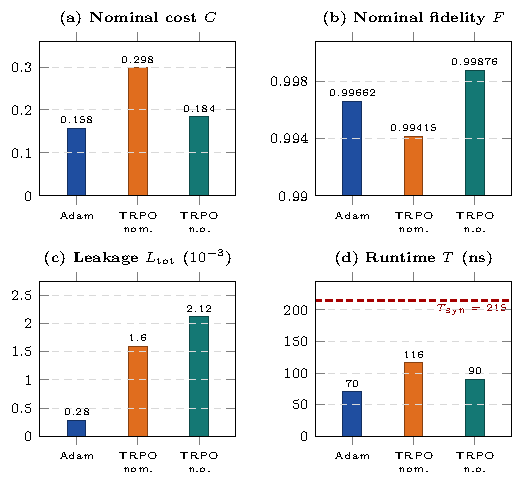
\includegraphics[width=\columnwidth]{single_target_comparison_v2.pdf}
\caption{Nominal comparison on $\Ntgt{2.2}{\pi/2}$ of the Adam baseline at its best horizon, the
nominal TRPO controller and the noise-optimized TRPO controller; values are those of
Table~\ref{tab:single}. (a) Total cost. (b) Nominal fidelity. (c) Total leakage. (d) Effective
runtime, with the gate-synthesis reference $\Tsyn=215\ns$ marked. Both TRPO controllers produce
genuinely high-quality solutions, but the direct optimizer dominates the nominal agent on all four
deterministic metrics, and every analog solution is well inside $\Tsyn$.}
\label{fig:singlebar}
\end{figure}

The comparison that matters for the rest of the paper is the third row against the first. On this
deterministic benchmark the direct optimizer beats the policy-gradient controller simultaneously in
cost ($1.89\times$), runtime ($1.66\times$), leakage ($5.67\times$) and, marginally, fidelity
($2.5\times10^{-3}$ absolute). This is not a defect of the RL formulation; it is a delimitation of what
it should be expected to deliver. When the model is known exactly and the objective is smooth and
differentiable, direct gradient methods are extremely effective on fixed-target closed-system pulse
design~\cite{Khaneja2005,Koch2022}, and nothing about policy optimization changes that. It also means
the baseline against which the robustness claims will be tested is a strong one rather than a
strawman.

The noise-optimized agent is the interesting case. It attains the \emph{highest} nominal fidelity of
all four solutions while also being the controller trained under perturbations --- so whatever
robustness it acquires is not bought by sacrificing nominal quality. Its leakage is the largest of the
set, which is consistent with a policy that hedges against amplitude fluctuations rather than driving
the multilevel dynamics as tightly as possible.

% =========================================================================
\section{Robustness under stochastic control noise}
\label{sec:robust}

\subsection{Evaluation protocol}

Each stored control plan is executed under the noise model of Sec.~\ref{sec:noise} on a dense grid of
$3401$ noise strengths spanning $\snoise\in[0.1,3.5]\MHz$ in steps of $0.001\MHz$, with $60$
independent realizations at each point --- about $2\times10^5$ noisy rollouts per controller. Sixty
samples give a noisy point estimate, so the curves are read through an exponentially weighted moving
average along the $\snoise$ axis (span $50$ for the mean, $80$ for the variance). This is not
cosmetic smoothing of sparse data: because neighbouring $\snoise$ values differ by $0.001\MHz$, the
average pools thousands of statistically comparable realizations, and the underlying scatter is
retained in the figures. Beyond this smoothing, no post-processing of any kind is applied: every
curve below is the direct Monte Carlo output of the evaluation pipeline.

An important detail of the comparison is that the Adam plan carried into this section is the one
selected under the \emph{noisy} training objective (Table~\ref{tab:single}), so the baseline is itself
noise-aware. The comparison is thus between a noise-aware direct optimizer and a noise-trained policy,
not between a robust method and a nominal one.

\begin{figure*}[t]
\centering
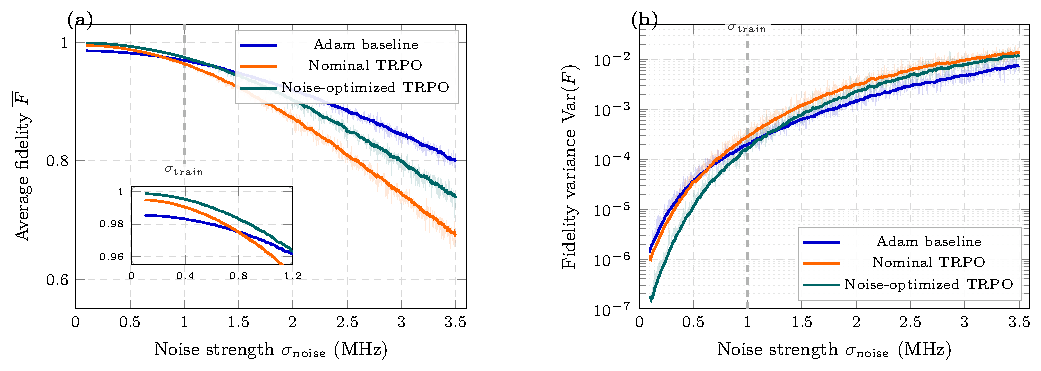
\includegraphics[width=\textwidth]{robustness_v2.pdf}
\caption{Robustness on $\Ntgt{2.2}{\pi/2}$. (a) Average fidelity $\Fbar(\snoise)$ over
$\snoise\in[0.1,3.5]\MHz$, with the low-noise regime magnified in the inset. (b) Fidelity variance on
a logarithmic axis. Solid lines are exponentially weighted moving averages along the noise axis
(spans $50$ and $80$); the underlying Monte Carlo scatter is visible behind them. The dashed vertical
line marks the training noise $\strain=1\MHz$. The noise-optimized agent is above the nominal agent in
(a) and below it in (b) at every noise strength, but it crosses the noise-aware Adam baseline at
$\snoise\approx1.3\MHz$ in the mean and $\approx1.2\MHz$ in the variance, beyond which the direct
optimizer is both more accurate and more stable.}
\label{fig:robust}
\end{figure*}

\subsection{Average fidelity and variance}

All three controllers degrade monotonically with noise, as they must; the question is how fast, and
relative to whom. Figure~\ref{fig:robust} separates two comparisons that the original framing tends to
merge, and they give different answers.

The first is the controlled comparison between the two TRPO agents, which differ \emph{only} in the
distribution of trajectories seen during training. Here the result is unambiguous and holds without
exception: the noise-trained policy has higher average fidelity and lower fidelity variance than the
deterministically trained policy at every one of the $3401$ noise strengths evaluated. Whatever is
responsible cannot be reinforcement learning as such, since both agents use it; it can only be
stochastic training.

The second is the comparison against the noise-aware Adam baseline, and here the picture is
qualitatively different. The noise-trained policy leads only at low noise. The mean-fidelity curves
cross at
\begin{equation}
\snoise^{\times}\approx1.29\MHz,
\label{eq:crossover}
\end{equation}
and the variance curves cross slightly earlier, at $\approx1.19\MHz$; beyond these points the direct
optimizer is simultaneously more accurate and more stable, and the gap widens monotonically. The
noise-trained policy is the best of the three controllers on only $35\%$ of the tested range in mean
fidelity and $32\%$ in variance --- namely the part at and below the training noise.

Table~\ref{tab:robust} makes both effects quantitative.

\begin{table}[t]
\caption{Robustness at representative noise strengths for the Adam baseline, the nominal TRPO agent
(nom.) and the noise-optimized TRPO agent (n.o.). $\Fbar$ is the channel average fidelity,
Eq.~\eqref{eq:favg}; the last two columns give infidelity ratios
$(1-\Fbar_{X})/(1-\Fbar_{\mathrm{n.o.}})$ in the upper block and variance ratios
$\mathrm{Var}(F)_{X}/\mathrm{Var}(F)_{\mathrm{n.o.}}$ in the lower block. Noise strengths $\snoise$ are
in MHz; all values are EWMA estimates over the dense noise grid. Ratios below unity mark the regime,
above $\snoise\approx1.3\MHz$, in which the direct optimizer overtakes the noise-trained policy.}
\label{tab:robust}
\footnotesize
\begin{ruledtabular}
\begin{tabular}{cccccc}
 & \multicolumn{3}{c}{$\Fbar$} & \multicolumn{2}{c}{infidelity ratio}\\
\cline{2-4}\cline{5-6}
$\snoise$ & Adam & nom. & n.o. & nom./n.o. & Adam/n.o.\\
\colrule
0.1 & 0.9857 & 0.9950 & 0.9987 & 3.76 & 10.88\\
0.5 & 0.9816 & 0.9874 & 0.9930 & 1.81 & 2.64\\
1.0 & 0.9691 & 0.9631 & 0.9744 & 1.44 & 1.21\\
1.5 & 0.9480 & 0.9238 & 0.9439 & 1.36 & 0.93\\
2.0 & 0.9193 & 0.8722 & 0.9020 & 1.31 & 0.82\\
3.0 & 0.8453 & 0.7449 & 0.7999 & 1.28 & 0.77\\
3.5 & 0.7989 & 0.6764 & 0.7381 & 1.24 & 0.77\\
\colrule
\multicolumn{6}{l}{\textit{Fidelity variance} $\mathrm{Var}(F)$ \textit{and ratios}}\\
\colrule
0.1 & $1.7\times10^{-6}$ & $1.2\times10^{-6}$ & $1.8\times10^{-7}$ & 6.56 & 9.67\\
1.0 & $2.0\times10^{-4}$ & $2.9\times10^{-4}$ & $1.7\times10^{-4}$ & 1.76 & 1.20\\
2.0 & $1.5\times10^{-3}$ & $3.1\times10^{-3}$ & $2.3\times10^{-3}$ & 1.37 & 0.65\\
3.5 & $7.6\times10^{-3}$ & $1.4\times10^{-2}$ & $1.2\times10^{-2}$ & 1.14 & 0.64\\
\end{tabular}
\end{ruledtabular}
\end{table}

Against the nominal agent the improvement is present everywhere but shrinks with noise: the infidelity
ratio falls from $3.76$ at $0.1\MHz$ to $1.44$ at $1\MHz$ and $1.24$ at $3.5\MHz$, and the variance
ratio from $6.56$ to $1.76$ to $1.14$. Against the Adam baseline the ratios cross unity between $1$ and
$1.5\MHz$ and then invert: at $3.5\MHz$ the direct optimizer has $0.77$ times the infidelity and
$0.64$ times the variance of the noise-trained policy.

The largest ratios sit at the lowest noise, and they are the least informative ones. At
$\snoise=0.1\MHz$ the comparison is dominated by the different \emph{nominal} operating points of the
three stored plans (Table~\ref{tab:single}) rather than by differential robustness. The
experimentally relevant statement is the one at $\snoise\approx1\MHz$, where the noise-trained policy
leads the nominal agent by $1.44\times$ in infidelity --- a real and systematic improvement, but one to
two orders of magnitude smaller than the gains reported in Ref.~\cite{Niu2019}.

A nominal-independent summary is how much fidelity each controller loses across the whole sweep,
$\Delta\Fbar=\Fbar(0.1\MHz)-\Fbar(3.5\MHz)$:
\begin{align}
\Delta\Fbar_{\text{Adam}}=0.187
&<\Delta\Fbar_{\text{noise-opt.}}=0.261
\nonumber\\
&<\Delta\Fbar_{\text{nominal}}=0.319 .
\label{eq:degradation}
\end{align}
Stochastic training reduces the loss of the RL controller by $18\%$ relative to deterministic
training. It does not, however, make it the slowest-degrading controller: that is the noise-aware
direct optimizer, by a clear margin.

\subsection{Interpretation}

Three conclusions follow, and they are more sharply delimited than a single benchmark number would
suggest.

First, robustness is genuinely learned rather than inherited. The two TRPO agents share architecture,
objective and algorithm, and differ only in the environment they were trained in; the noise-trained
one is better on both metrics at every noise strength. The improvement is also two-dimensional --- mean
fidelity is not bought at the cost of shot-to-shot stability --- which is what one expects if the policy
has converged onto trajectories intrinsically less sensitive to amplitude fluctuations and to the
unactuated anharmonicity parameter.

Second, and this is the main qualification our data impose, the learned robustness is \emph{local to
the training scale}. The agent was trained at $\strain=1\MHz$, and Eq.~\eqref{eq:crossover} places its
advantage over a noise-aware direct optimizer at roughly $1.3\times$ that value. Below the crossover
the policy exploits structure specific to the perturbation magnitude it was exposed to; above it, that
specialization stops paying, and a controller that simply optimizes the same objective directly
extrapolates better. This is a natural failure mode for distributionally trained policies, and it is
invisible if robustness is quoted at a single operating point --- which is precisely how it is usually
quoted.

Third, the practical regime in which the learning formulation earns its cost is therefore narrow but
well defined. It is the regime where the perturbation model is known well enough to be simulated
\emph{and} the deployed noise is close to the modelled noise. Where the noise level is uncertain, or
where it may exceed the training scale by more than about $30\%$, a strong noise-aware direct
optimizer is the safer choice on this problem. This does not contradict the mechanism the UFO
framework proposes; it bounds the conditions under which the mechanism is worth its computational
cost.

% =========================================================================
\section{Runtime across the gate family}
\label{sec:runtime}

\subsection{Curriculum protocol}

To test hardware efficiency beyond a single target we sweep the one-parameter subfamily
\begin{equation}
\Utgt(\alpha)=\Ntgt{\alpha}{\pi/2},\qquad \alpha\in[0,\pi],
\label{eq:runtimefamily}
\end{equation}
in $21$ steps of $0.157$. Rather than retraining from scratch at each point, the best checkpoint
obtained at one $\alpha$ initializes training at the next --- a curriculum that exploits continuity in
target space, in the spirit of the transfer strategy of Ref.~\cite{Niu2019}. Training at each target
stops when the cost falls below $0.40$ or after $150$ iterations. The environment remains stochastic
at $\strain=1\MHz$, so the runtimes reported here belong to robustly trained controllers, not to
nominal ones.

As a no-transfer control we also sweep the same family with the Adam baseline, optimizing each of $33$
targets independently over the horizon grid of Table~\ref{tab:config}. This separates two effects that
the curriculum conflates: how uniformly hard the analog control problem is across the family, and how
much is gained by reusing previously learned structure.

\begin{figure*}[t]
\centering
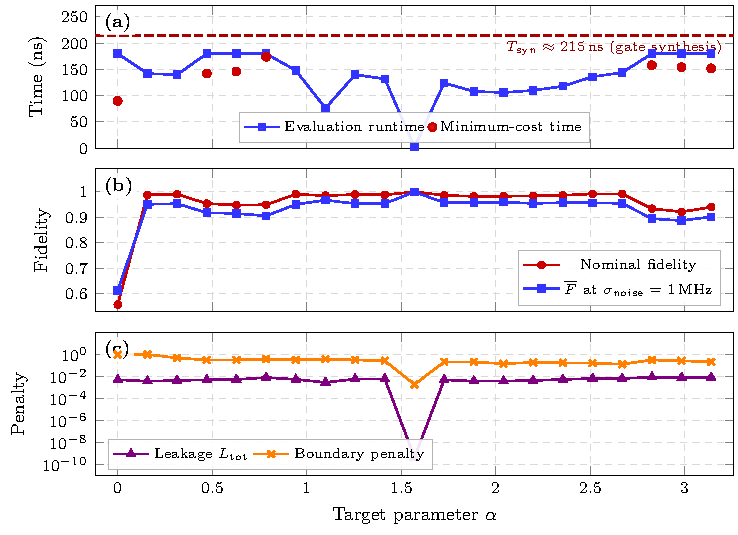
\includegraphics[width=0.70\textwidth]{runtime_vs_alpha_v2.pdf}
\caption{Curriculum sweep over $\Ntgt{\alpha}{\pi/2}$. (a) Final evaluation runtime and the
minimum-cost time reached within the same training phase; the two separate exactly where the optimizer
fails to push the cost below the early-termination threshold and the rollout runs to the $180\ns$
ceiling. The dashed line is the optimal gate-synthesis reference $\Tsyn\approx215\ns$, which the
analog controller stays below across the entire family. (b) Nominal fidelity and average fidelity
under $\snoise=1\MHz$. (c) Leakage and boundary penalties on a logarithmic axis. The fastest regions
are also the cleanest and the most robust.}
\label{fig:runtime}
\end{figure*}

\subsection{Runtime landscape}

The runtime profile is strongly structured rather than monotonic (Fig.~\ref{fig:runtime},
Table~\ref{tab:runtime}). Four regimes are visible: a cold-start point, an irregular low-$\alpha$
region, a broad central basin of fast and accurate solutions, and a degradation region approaching
$\alpha=\pi$.

The point $\alpha=0$ must be read separately. It is the only target not warm-started from a neighbour,
and it behaves like it: fidelity $0.558$, runtime saturated at $180\ns$, leakage $4.8\times10^{-3}$,
robust fidelity $0.613$. It measures cold-start difficulty, not family structure.

From $\alpha\approx0.157$ the curriculum enters its transferable regime, reaching $142$ and $140\ns$
with fidelities above $0.988$. The interval $\alpha\in[0.47,0.79]$ is then harder again --- runtime
returns to the $180\ns$ ceiling, fidelity falls to $0.948$--$0.954$ and robust fidelity to
$0.906$--$0.918$ --- and, tellingly, this region also shows visibly larger leakage and boundary costs.
The difficulty is dynamical, not merely temporal.

The central basin $\alpha\in[1.1,2.4]$ is the main result. Targets are solved in $76$--$140\ns$, with
the best stretch between $\alpha\approx1.88$ and $2.36$ giving $108$, $106$, $110$ and $118\ns$ at
nominal fidelity above $0.982$ and robust fidelity $0.954$--$0.959$. The speedup is not bought with
accuracy: the fast region is also the accurate and robust region.

At the centre, $\alpha=\pi/2$ is a singular point. The controller terminates after $2\ns$ with
fidelity $0.999999$, leakage $4\times10^{-10}$, and robust fidelity still $0.9994$ at $\snoise=1\MHz$
--- and it needs a single curriculum iteration to get there. This is not a fluctuation; it is a
dynamical alignment, discussed below.

Beyond the basin, $\alpha\in[1.73,2.67]$ remains favourable ($124$--$144\ns$, fidelity
$0.982$--$0.992$), and only for $\alpha\gtrsim2.83$ does the sweep degrade clearly, with runtimes back
at $180\ns$ and fidelity falling to $0.921$--$0.940$.

A diagnostic hidden in Fig.~\ref{fig:runtime}(a) is worth extracting. For well-converged targets the
final runtime coincides with the minimum-cost time reached during the phase. In the hard regions it
does not: near $\alpha\approx0.47$ and $0.63$ the lowest-cost trajectory occurs at $142$--$146\ns$
while the final rollout still ends at $180\ns$, and the same happens near $\alpha\gtrsim2.83$ with
minima at $152$--$158\ns$. The hard regions are therefore not regions where short solutions fail to
exist --- the agent visits them transiently --- but regions where short solutions fail to be
\emph{stabilized} under the full objective.

\subsection{Comparison with gate synthesis}

\begin{table}[t]
\caption{Curriculum runtime sweep over $\Ntgt{\alpha}{\pi/2}$. $T$ is the final evaluation runtime,
$T_{\min}$ the minimum-cost time within the same phase, and the speedup is $\Tsyn/T$ with
$\Tsyn=215\ns$. Rows in the central basin are the fastest.}
\label{tab:runtime}
\begin{ruledtabular}
\begin{tabular}{cccccc}
$\alpha$ & $T$ (ns) & $T_{\min}$ (ns) & $F^{\mathrm{nom}}$ & $\Fbar_{\sigma=1}$ & $\Tsyn/T$\\
\colrule
0.000 & 180 & 90  & 0.5577 & 0.6133 & 1.19\\
0.157 & 142 & 142 & 0.9880 & 0.9510 & 1.51\\
0.314 & 140 & 140 & 0.9905 & 0.9533 & 1.54\\
0.471 & 180 & 142 & 0.9538 & 0.9179 & 1.19\\
0.628 & 180 & 146 & 0.9480 & 0.9149 & 1.19\\
0.785 & 180 & 174 & 0.9492 & 0.9055 & 1.19\\
0.942 & 148 & 148 & 0.9905 & 0.9504 & 1.45\\
1.099 & \textbf{76}  & 76  & 0.9850 & 0.9674 & \textbf{2.83}\\
1.256 & 140 & 140 & 0.9894 & 0.9535 & 1.54\\
1.413 & 132 & 132 & 0.9880 & 0.9542 & 1.63\\
1.571 & \textbf{2} & 2 & 0.99999 & 0.9994 & \textbf{107.5}\\
1.727 & 124 & 124 & 0.9861 & 0.9575 & 1.73\\
1.884 & 108 & 108 & 0.9821 & 0.9582 & 1.99\\
2.041 & 106 & 106 & 0.9825 & 0.9595 & 2.03\\
2.198 & 110 & 110 & 0.9837 & 0.9545 & 1.95\\
2.355 & 118 & 118 & 0.9863 & 0.9573 & 1.82\\
2.512 & 136 & 136 & 0.9919 & 0.9567 & 1.58\\
2.669 & 144 & 144 & 0.9918 & 0.9547 & 1.49\\
2.826 & 180 & 158 & 0.9340 & 0.8944 & 1.19\\
2.983 & 180 & 154 & 0.9213 & 0.8872 & 1.19\\
3.140 & 180 & 152 & 0.9400 & 0.9020 & 1.19\\
\end{tabular}
\end{ruledtabular}
\end{table}

Measured against $\Tsyn\approx215\ns$, the analog controller is faster \emph{everywhere} in the family.
Even the hardest edge points, where the controller saturates the $180\ns$ ceiling, retain a $35\ns$
margin, i.e.\ about $16\%$. That the advantage survives precisely where the optimization is most
difficult is the more robust half of the claim.

In the central basin the margin is systematic rather than marginal: for $\alpha\in[1.73,2.36]$ the
learned runtimes of $106$--$124\ns$ correspond to reductions of $42$--$51\%$, at nominal fidelity
$0.982$--$0.986$ and robust fidelity $0.955$--$0.959$. At $\alpha\approx1.10$ the runtime drops to
$76\ns$, a factor $2.8$, still above $0.98$ nominal and $0.96$ robust fidelity. And at $\alpha=\pi/2$
the $2\ns$ solution formally corresponds to a factor of order $100$ --- a number that should not be
read as a family-level statement, but which does demonstrate something conceptually sharp: the
compilation overhead of discrete synthesis is not a lower bound on physical execution time, only on
execution time \emph{through a prescribed gate alphabet}.

That distinction deserves emphasis, because it is easy to overclaim here. The synthesis benchmark is
optimal within a circuit model over a fixed elementary gate library, whereas the analog controller
optimizes in the continuous Hamiltonian-control space. The two solve related but different problems.
Nothing in these results says that a quantum speed limit has been beaten. What they do say is that
when the hardware offers a rich native interaction and sufficiently flexible pulse shaping, the
shortest useful implementation of a target gate need not coincide with its shortest decomposition into
universal primitives --- which is the notion of efficiency that matters for near-term devices.

\subsection{What the runtime comparison actually measures}
\label{sec:runtimecaveat}

\begin{figure}[t]
\centering
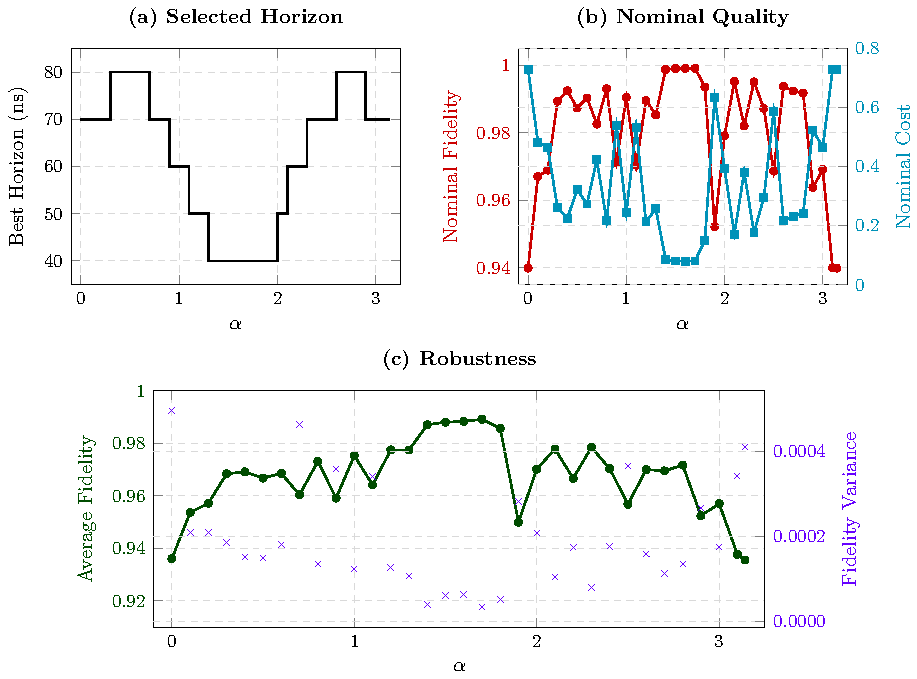
\includegraphics[width=\columnwidth]{adam_family_sweep.pdf}
\caption{No-transfer control: the Adam baseline swept independently over $33$ targets of
$\Ntgt{\alpha}{\pi/2}$. (a) Selected horizon versus $\alpha$. (b) Nominal fidelity and cost.
(c) Average fidelity at $\snoise=1\MHz$ and the corresponding variance. Difficulty is markedly
non-uniform across the family even without any policy learning, with the easiest region in the centre
--- the same region the curriculum finds easiest.}
\label{fig:adamfamily}
\end{figure}

Two observations complicate the reading of Sec.~\ref{sec:runtime} and should be stated explicitly.

First, the independently optimized Adam baseline is \emph{faster than the curriculum controller across
the family}. Its selected horizons span $40$--$80\ns$ with a median of $70\ns$ (Fig.~\ref{fig:adamfamily}),
against $76$--$180\ns$ and a median near $140\ns$ for the curriculum TRPO sweep, at comparable nominal
fidelity (median $0.987$ versus $0.985$) and comparable or better robustness at $\snoise=1\MHz$ (median
$0.969$ versus $0.953$). Every one of the $33$ Adam solutions lies below $\Tsyn$, with a median
speedup of $3.1\times$ against the $1.5$--$2.0\times$ typical of the curriculum. The single point at
which the RL controller is decisively better is the singular $\alpha=\pi/2$.

The conclusion we draw is therefore narrower than a straightforward reading of Fig.~\ref{fig:runtime}
would support: the runtime advantage over compiled gate synthesis is a property of \emph{direct analog
optimization on this hardware model}, not a benefit conferred by reinforcement learning. Both
optimizers exploit the native exchange interaction; the alignment argument of
Sec.~\ref{sec:physicalinterp} explains the shape of both curves, and the family-resolved structure of
Fig.~\ref{fig:adamfamily} closely tracks that of Fig.~\ref{fig:runtime}.

Second, the curriculum runtimes are partly an artifact of the stopping rule. Training at each target
halts as soon as the UFO cost drops below the advancement threshold $0.40$, and the evaluation costs
in Table~\ref{tab:runtime} show the consequence directly: every converged phase sits in the narrow
band $C\in[0.393,0.400]$, immediately beneath the threshold, while the failures sit above $0.94$. The
agent therefore stops improving the moment it becomes good enough to advance, and has no incentive to
shorten the pulse further. The curriculum runtimes should be read as \emph{times sufficient to reach a
fixed cost target} under a bounded budget, not as the shortest times the policy could achieve. A
tighter threshold would very likely move the curve down; we did not run that sweep, and we flag it as
the obvious next test rather than assuming its outcome.

\subsection{Physical interpretation}
\label{sec:physicalinterp}

The structure of Table~\ref{tab:runtime} is not an artifact of the optimizer. The native entangling
term of Eq.~\eqref{eq:hrwa} is the exchange coupling
$g(t)(\hat a_2^\dagger\hat a_1+\hat a_1^\dagger\hat a_2)$, whose action on the computational subspace
is aligned with the $XX+YY$ sector --- exactly the sector that carries the $\alpha$ dependence of the
target family, Eq.~\eqref{eq:family}. When the required nonlocal content can be generated largely
along that native direction, the controller does not have to fight the hardware: it can accumulate the
entangling action directly and use the local channels only to shape phases, suppress leakage and
satisfy the boundary constraints. Short runtimes in that regime are physically expected, not
fortuitous.

This explains why the favourable region sits in the middle of the interval rather than at its edges,
and why runtime, leakage and robustness co-vary across the sweep. In the basin the pulse needs only
modest corrective excursions in the local channels, the boundary term stays moderate and the leakage
proxy stays controlled; the region that is fastest is also the one that is easiest to control
reliably. Toward the edges the target is less directly compatible with the native evolution, the
controller must lean harder on detuning and microwave components to steer the dynamics while
suppressing population transfer, and the consequence is twofold: longer sequences, because the correct
effective nonlocal action takes longer to accumulate without violating the penalties; and more fragile
ones, because a longer, more structured pulse is exposed to perturbations for longer. Both effects are
visible in Fig.~\ref{fig:runtime}.

The $\alpha=\pi/2$ point should be read in the same spirit but with more caution. Its collapse to
$2\ns$ indicates a particularly favourable local-equivalence configuration within the family, in which
the desired transformation is reached almost immediately once the controller is placed in the right
dynamical sector. It is a statement about that point, not a generic realizability claim for two-qubit
gates. The transferable conclusion is the pattern rather than the extremum: runtime minima occur where
physical compatibility with the native generator is highest.

% =========================================================================
\section{Discussion}
\label{sec:discussion}

\subsection{What reproduces}

Two of the central claims of Ref.~\cite{Niu2019} reproduce cleanly under an independent
implementation.

The first is that robustness against stochastic control errors is a \emph{trainable} property rather
than a post-hoc diagnostic. Our noise-optimized agent beats the otherwise identical nominal agent in
both average fidelity and fidelity variance at every noise strength in $\snoise\in[0.1,3.5]\MHz$, and
loses $18\%$ less fidelity across the sweep, Eq.~\eqref{eq:degradation}. Because the two agents differ
only in the training distribution, the attribution is unambiguous. This is the claim of
Ref.~\cite{Niu2019} that survives most cleanly.

The second is the physical mechanism behind the runtime advantage. Analog control is faster than
optimal gate synthesis over the entire family, and --- as predicted by the alignment argument --- the
gains are largest exactly where the target is closest to the native exchange interaction, with a
singular point at $\alpha=\pi/2$. Both optimizers reproduce this structure, which supports not only the
trend but the explanation offered for it.

\subsection{What does not}

Three quantitative discrepancies are worth stating plainly.

\emph{Nominal superiority does not hold.} On $\Ntgt{2.2}{\pi/2}$ the direct Adam baseline outperforms
the nominal TRPO controller on every deterministic metric (Table~\ref{tab:single}). Ref.~\cite{Niu2019}
compares against an SGD baseline and reports a large margin in favour of policy optimization; with a
well-tuned Adam optimizer acting on the same Hamiltonian and the same objective, the margin reverses.
We take this to mean that part of the originally reported gap reflects the strength of the baseline
rather than an intrinsic property of policy-gradient control.

\emph{The robustness margin is much smaller, and it does not extend past the training scale.} Against
$10\times$ (versus noise-free RL) and $100\times$ (versus a gradient baseline) improvements in average
gate infidelity, we find $1.44\times$ and $1.21\times$ at $\snoise=1\MHz$, the scale the original work
itself identifies as experimentally representative (Table~\ref{tab:robust}). Ratios approaching an
order of magnitude appear only below $\snoise\approx0.2\MHz$, where they largely reflect the different
nominal operating points of the compared plans rather than differential robustness. More consequential
than the magnitude is the crossover of Eq.~\eqref{eq:crossover}: above $\snoise\approx1.3\MHz$ the
noise-aware Adam baseline overtakes the noise-trained policy in \emph{both} metrics and stays ahead.
The original comparison is drawn against a gradient baseline optimized without noise awareness and
reported at a single noise level, a protocol that cannot expose this behaviour. We regard the
locality of the learned robustness, rather than its size, as the most important qualification our
reproduction adds.

\emph{The runtime advantage is non-uniform, and it is not attributable to reinforcement learning.}
Rather than a uniform factor-ten improvement, we find a structured landscape spanning $1.19\times$ at
the edges to $2.83\times$ in the basin, plus one singular point; and regions exist where the controller
transiently discovers short solutions and then fails to stabilize them. More importantly, the
independently optimized direct baseline is faster than the curriculum controller across the family
(median $3.1\times$ versus $1.5$--$2.0\times$ over $\Tsyn$) at comparable fidelity and robustness
(Sec.~\ref{sec:runtimecaveat}). The speedup over compiled synthesis is therefore evidence for analog
pulse-level control, not for the policy-gradient method that produced one instance of it. Part of the
gap is a stopping-rule artifact --- the curriculum halts at a fixed cost threshold --- but that
qualification cuts against the RL runtime claim rather than for it.

\subsection{Why the discrepancies are unsurprising}

None of this invalidates the framework, and some of it is simply what independent reimplementation
means. The two studies differ in discretization, filtering pipeline, stopping rules, curriculum
schedule, training budget and evaluation protocol, and the underlying optimization problem is
high-dimensional and non-convex; exact numerical coincidence is not the appropriate standard.

The parameter studies of Sec.~\ref{sec:modelsel} support this reading concretely. Performance depends
measurably but non-monotonically on the actor--critic architecture, and interpretably on the UFO
weights: too small a fidelity weight degrades control quality outright, while too strong a boundary
penalty reduces leakage at the cost of destabilizing the fidelity--robustness trade-off. That the
original choices sit close to the best region in an independent implementation is a nontrivial check
in their favour. That the surrounding landscape is not flat is why quantitative claims from this class
of experiment should be quoted with their configuration.

\subsection{Limitations}

The study is simulation-based. The model is physically motivated but truncated to three levels per
mode under a rotating-wave description, and real devices add transfer-function nonlinearities,
spurious modes, drift and measurement constraints that are not represented. The noise model is
Gaussian and white, applied to control amplitudes and to $\eta$; it does not cover quasi-static drift,
temporally correlated noise, or open-system decoherence, so the robustness reported here should be
read as robustness \emph{to that model}. Whether it generalizes to qualitatively different
perturbations is the single most valuable open question left by this work. Finally, the comparison is
between one RL framework and one strong direct optimizer; it is not a ranking of control
methodologies, and does not include automatic-differentiation GRAPE/Krotov variants, differentiable
programming controllers, or model-based RL~\cite{Khalid2023}.

\subsection{Relation to subsequent work}

Read from the present vantage point, the lasting contribution of Ref.~\cite{Niu2019} looks less like a
particular optimizer and more like a demonstration that robust analog control can be posed as a
learning problem with leakage-aware costs and stochastic perturbations. The literature since has
refined that in two directions that our results make concrete. Model-free and hardware-interacting
schemes reduce model bias by adapting on the device itself~\cite{Sivak2022}; and model-based or hybrid
methods address the sample inefficiency that makes pure model-free RL expensive in
practice~\cite{Khalid2023}. Our results sharpen the case for both. A direct optimizer wins the nominal
problem and wins again once the deployed noise exceeds the modelled noise; the learned policy wins in
between. Since a real device's noise is known only approximately, that is an argument for hybrid
workflows rather than for either extreme: use direct optimization or a learned policy to generate
physically informed pulses, then refine them in closed loop against the device, where the effective
perturbation distribution is the device's own rather than a modelled
one~\cite{Vetter2024,Glaser2025,Wang2024}.

% =========================================================================
\section{Conclusion}
\label{sec:conclusion}

We have independently reimplemented and assessed the UFO framework for robust analog two-qubit gate
design on a multilevel gmon model, including the second-order TSWT leakage bound, the exact bandwidth
filter, and TRPO training in a stochastic control environment.

The framework's core mechanism survives independent scrutiny. Embedding the perturbation model in the
training environment produces a controller that is measurably more accurate \emph{and} more
reproducible under control noise than the identical architecture trained deterministically, at every
noise strength tested, losing $18\%$ less fidelity across the sweep. The runtime advantage of analog
control over optimal gate synthesis is likewise real across the whole family $\Ntgt{\alpha}{\pi/2}$,
and is largest exactly where the target aligns with the native exchange interaction --- confirming the
physical mechanism, not just the trend.

The reproduction also narrows the claims in three ways. Policy-gradient control is not a better
nominal optimizer than a well-tuned direct gradient method on a fixed, exactly known target. The
runtime advantage over compiled synthesis, while real and physically interpretable, belongs to analog
pulse-level control rather than to the learning method: an independently optimized direct baseline is
faster across the family, and only the singular point $\alpha=\pi/2$ favours the policy. And, most
consequentially, the robustness advantage is local: measured against a direct optimizer given the same
noise awareness, the noise-trained policy leads only up to $\snoise\approx1.3\MHz$, about $1.3$ times
the noise it was trained on, and falls behind in both mean fidelity and variance beyond that.

That last result is the one we would most like to see tested elsewhere. It suggests that the useful
question about noise-aware RL for quantum control is not how large its advantage is at the design
noise level, but how far in perturbation space that advantage extends --- a quantity that a
single-operating-point benchmark cannot reveal, and that determines whether such controllers are
usable on a device whose noise is only approximately known. The natural companion experiment is the
one our noise model does not reach: whether robustness trained on Gaussian amplitude fluctuations
transfers at all to quasi-static drift, colored noise, parameter mismatch and decoherence. Together
those two axes, magnitude and mechanism, separate a policy that has learned distribution-specific
compensation from one that has found a genuine control regularity.

% =========================================================================
\section*{Data availability}

The robustness curves of Fig.~\ref{fig:robust} and Table~\ref{tab:robust} are the direct Monte Carlo
outputs of the evaluation pipeline on the grid of Table~\ref{tab:config}, with no post-processing
other than the exponentially weighted smoothing stated in Sec.~\ref{sec:robust}; raw and smoothed
columns are both retained in the released data. The runtime sweep of Table~\ref{tab:runtime} and the
model-selection sweeps of Sec.~\ref{sec:modelsel} are likewise reported as produced by the training
scripts.

The material needed to reproduce every number in this paper consists of the simulation code
implementing Secs.~\ref{sec:framework} and \ref{sec:methods}, the stored control plans for the four
controllers of Table~\ref{tab:single}, the per-target logs of the curriculum and Adam family sweeps,
and the per-seed records of the two model-selection sweeps. Together with the complete parameter set
given in Table~\ref{tab:config}, these are sufficient to regenerate all figures and tables from
scratch. They are available from the author on request and are being prepared for public deposit.

% =========================================================================
\begin{acknowledgments}
I thank Prof.\ Morten Hjorth-Jensen and Prof.\ Davide Emilio Galli for their supervision and for many
discussions that shaped this work. This study was carried out as part of a Bachelor's thesis at the
Department of Physics, Universit\`a degli Studi di Milano. AI-based tools were used as auxiliary
instruments for code drafting and debugging, literature search, and stylistic revision; all
derivations, modeling assumptions, numerical methodology, experimental design and results were
independently verified by the author.
\end{acknowledgments}

% =========================================================================
\appendix

\section{The TSWT coherent leakage bound}
\label{app:tswt}

We summarize the derivation of Eq.~\eqref{eq:leakbound}. Starting from the decomposition
Eq.~\eqref{eq:decomp} in the regime $\epsilon/\Delta\ll1$, one seeks an anti-Hermitian generator
$\hat S(t)=\epsilon\hat S_1+\epsilon^2\hat S_2+\dots$ such that the transformed Hamiltonian
Eq.~\eqref{eq:tswt} is block-diagonal to the desired order. Order by order, the block-off-diagonal
components must satisfy
\begin{equation}
[\hat H_0,\hat S_1]=-\hat H_2,\qquad
[\hat H_0,\hat S_2]=-\bigl([\hat H_1,\hat S_1]-i\dot{\hat S}_1\bigr)_{\mathrm{od}},
\label{eq:generators}
\end{equation}
which are solved elementwise on the off-diagonal blocks by dividing by the subspace energy differences
$E_\alpha-E_{\alpha'}$; the assumption $\epsilon/\Delta\ll1$ is what makes these divisions safe. After
second order the residual block-off-diagonal Hamiltonian is
\begin{equation}
H_{\mathrm{od}}^{(3)}=[\hat H_1,\hat S_2]+\tfrac{1}{3}\bigl[[\hat H_2,\hat S_1],\hat S_1\bigr]-i\dot{\hat S}_2
=O\!\left(\frac{\epsilon^3}{\Delta^2}\right).
\label{eq:hod3}
\end{equation}
The leakage amplitude out of $\Omega_0$ over $[0,T]$ is then an interaction-picture integral of
$\Hod$ against a rapidly oscillating phase $e^{i\int\Delta dt}$. Repeated integration by parts
converts this into boundary terms, which pick up $\|\Hod\|/\Delta$ at $t=0$ and $t=T$, plus a residual
integral controlled by the second derivative of $\Hod$ divided by $\Delta^2$. Collecting these gives
Eq.~\eqref{eq:leakbound}.

The two contributions dominate in complementary regimes: for slow, off-resonant modulation the
boundary terms dominate, and for faster on-resonant modulation the derivative term does. This is why
the bound is usable as a single penalty across the operating range rather than only in one limit.

\section{Algorithmic details}
\label{app:algo}

\paragraph*{Environment step.}
Given the current observation and propagator: map the action to physical controls; apply the bandwidth
filter Eq.~\eqref{eq:filter}; if stochastic training is enabled, sample Gaussian perturbations for
$g,\delta_{1,2},f_{1,2}$ and $\eta$ and wrap the phases modulo $2\pi$; build $H_t$ from
Eq.~\eqref{eq:hrwa}; propagate $U_{t+1}=e^{-iH_t\Delta t}U_t$ by exact diagonalization; update the
leakage estimator; evaluate the running cost Eq.~\eqref{eq:ufo} and reward $r=-C$; test the stopping
condition (time limit or cost threshold); emit the next observation Eq.~\eqref{eq:obs}.

\paragraph*{Incremental leakage estimator.}
At each step: decompose $H_t$ into $H_0,H_1,H_2$; solve Eq.~\eqref{eq:generators} for $S_1$; estimate
$\dot S_1$ from the stored previous value by finite differences; solve for $S_2$; estimate $\dot S_2$;
form $H_{\mathrm{od}}^{(3)}$ from Eq.~\eqref{eq:hod3} and symmetrize; take its spectral norm. The first
and last samples update the boundary contribution; the discrete second derivative, formed from the two
previous stored values, updates the integral contribution. Storing only the two previous states keeps
the estimator $O(1)$ per step.

\paragraph*{TRPO loop.}
Per iteration: collect a batch of stochastic rollouts in parallel workers; compute discounted returns
and generalized advantage estimates~\cite{Schulman2016GAE}; take the KL-constrained policy step
Eq.~\eqref{eq:trpo} by conjugate gradient with backtracking line search; refit the value network by
regression on the empirical returns; evaluate the deterministic policy in the nominal environment and
store the control plan if it improves on the best so far. Checkpoints and induced control plans are
saved every iteration, so that comparisons can be made at the level of the realized pulse rather than
only at the level of network weights.

\paragraph*{Adam baseline.}
For each candidate horizon: discretize the trajectory into $N_T=T/\Delta t$ steps; initialize the pulse
parameters; iterate simulate--evaluate--update for $400$ Adam steps; store the optimized plan and
re-evaluate it deterministically for cost, fidelity, leakage, boundary penalty and runtime. The best
horizon is selected on the re-evaluated metrics, not on the optimizer's internal objective --- a
distinction that matters here, since the noisy objective selects $60\ns$ while deterministic
re-evaluation selects $70\ns$.

% =========================================================================
\bibliographystyle{apsrev4-2}
\bibliography{references}

\end{document}
